\documentclass[20pt]{beamer}
\usepackage[orientation=portrait,size=a0,scale=1.8,debug]{beamerposter}
\mode<presentation>{\usetheme[articleid=WEPOPRPO21]{LNLS}}
\usepackage{chemformula}
\usepackage[utf8]{inputenc}
\usepackage[english]{babel} % required for rendering German special characters
\usepackage{siunitx} %pretty measurement unit rendering
\usepackage{hyperref} %enable hyperlink for urls
\usepackage{ragged2e}
\usepackage{calc}
\usepackage{datetime}
\newlength{\mylength}

\usepackage{array,booktabs,tabularx}
\newcolumntype{Z}{>{\centering\arraybackslash}X} % centered tabularx columns

\title{\huge Development of a Virtual Accelerator for Sirius}
\author{\underline{X. R. Resende}, A. H. C. Mukai, L. N. P. Vilela, I. Stevani}
\institute{Brazilian Synchrotron Light Laboratory (LNLS), Campinas, Brazil}
\date{\monthname \ \the\year}

\newlength{\abstractheight}
\setlength{\abstractheight}{15cm}

\newlength{\columnheight}
\setlength{\columnheight}{95cm}

\begin{document}
\begin{frame}
\begin{beamercolorbox}[center]{postercolumn}
	\begin{minipage}{\textwidth}
		\parbox[t][\abstractheight]{\textwidth}{
		\begin{myblock}{\textit{Abstract}}
		A virtual accelerator is being developed for Sirius, the new 4th generation synchrotron light source being built in Campinas, Brazil.
		The virtual accelerator is an on-line beam simulator which is integrated into EPICS control system.
		It consists on a command line interface server with a channel access (CA) layer and with an in-house developed tracking code library written in C++ for efficiency purpose.
		The purpose of such server is to facilitate early development and testing of high level applications for the control system.
		\end{myblock}
	}\end{minipage}
\end{beamercolorbox}
\begin{columns}
	\begin{column}{0.45\textwidth}
		\begin{beamercolorbox}[center]{postercolumn}
			\begin{minipage}{.98\textwidth}  % tweaks the width, makes a new \textwidth
				\parbox[t][\columnheight]{\textwidth}{ % must be some better way to set the height, width and textwidth simultaneously
					\begin{myblock}{VACA - Virtual Accelerator with Channel Access}
						\begin{itemize}
							\item VACA is written in Python3.
							\item High level programming language allows for rapid development
							\item Python language works as a binding layer between the two main core modules: a CA server and a tracking code for simulations.
							The python package PCasPy is used as the CA server module.
							\item PVs implemented in VACA have a prefix "VA-" indicating that they represent virtual process variables.
							\item Use of trackcpp: developed at LNLS by the accelerator physics group.
							\item Trackcpp is converted to Python package with Swig3.0
						\end{itemize}
						\begin{figure}
							\centering
							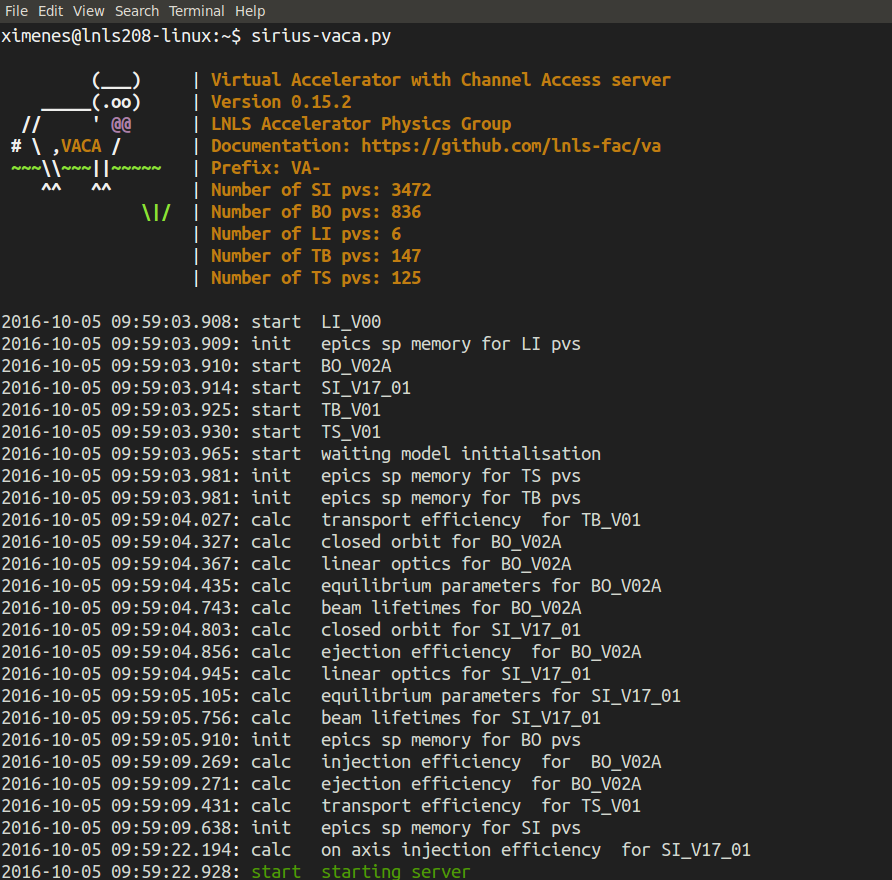
\includegraphics[width=1.0\textwidth]{../WEPOPRPO21f1.png}
							\caption{Screen printout of a command line terminal showing a running instance of VACA with the display of its banner and useful information.}
						\end{figure}
					\end{myblock}
		}\end{minipage}\end{beamercolorbox}
	\end{column}
	\begin{column}{.55\textwidth}
		\begin{beamercolorbox}[center]{postercolumn}
			\begin{minipage}{.98\textwidth} % tweaks the width, makes a new \textwidth
				\parbox[t][\columnheight]{\textwidth}{ % must be some better way to set the the height, width and textwidth simultaneously
					\begin{myblock}{Virtual IOCs}
					\begin{itemize}
					\item \textbf{si\_bpm,bo\_bpm,ts\_bpm,tb\_bpm}: they serve BPM positions that are read from VACA, adding emulated measurement fluctuations.
					\item \textbf{si\_current,bo\_current}: they provide simulated beam currents with fluctuations. Touschek, elastic and inelastic simulated lifetimes are affected by variations of associated parameters such as RF gap voltage and reduced acceptance due to closed orbit variations.
					\item \textbf{si\_ps,bo\_ps,ts\_ps,tb\_ps}: provide read/write access to PVs that correspond to power supplies with associated magnet excitation curves.
					\item \textbf{si\_rf,bo\_rf}: implement radio frequency process variables.
					\item \textbf{si\_tune}: emulation of the tune measurement IOC.
					\item \textbf{si\_beamsize, bo\_beamsize}: emulation of beam size measurement IOC.
					\end{itemize}
						\vspace{0.5cm}
					\end{myblock}\vfill
					\begin{myblock}{Conclusions}
					\begin{itemize}
					\item Details of the pulsed signals during injection and ejection processes need be considered.
					\item Approximate coupling expressions for beam size estimates should be substituted by Ohmi's envelop formalism\cite{ohmi} in trackcpp,
					\item A cleaner separation between VACA and vIOCS is in order. At this points a few excitation curves are implemented in VACA since it has not been decied yet where they will finally be located in the CS. They can either be moved to the IOCs, in case they should be moved to the vIOCS for the VA, or moved to some configuration database service.
					\item Considerations on moving from EPICS database records PCASPy for vIOCS developments. This may simplify the process of writing and deploying applications.
					\item Recently a few DISCS\cite{discs} services have been adopted. In particular, the use of its naming service allowed for a standardization of how to name devices and PVs. A major revision of PV names has taken place recently. VA should be modified to contemplate the new PV name standard.
					\end{itemize}
						\vspace{0.5cm}
					\end{myblock}\vfill
		}\end{minipage}\end{beamercolorbox}
	\end{column}
\end{columns}
\end{frame}
\end{document}
